\documentclass[11pt,a4paper]{article}
\usepackage[margin=2.2cm]{geometry}
\usepackage{booktabs}
\usepackage{graphicx}
\usepackage{siunitx}
\usepackage{enumitem}
\usepackage[font=small,labelfont=bf]{caption}
\usepackage[hidelinks]{hyperref}
\setlist{itemsep=2pt,topsep=4pt}
\sisetup{separate-uncertainty=true}

\title{Astronomical Bycatch: progress report}
\author{Huw Leggate}
\date{20 October 2026}

\begin{document}
\maketitle

\section{Summary}

The aim is to get light curves for the stars in archival images using the
new extraction API in our private EXOTIC fork (\texttt{exotic.extract}).
This report covers the first day of that work:

\begin{itemize}
  \item Code to search and download raw data from the ESO Science Archive,
        and to find archive sequences that cover a known transit.
  \item A pipeline that plate-solves frames locally against Gaia DR3, runs
        \texttt{extract\_sequence} on every usable star in the field, fits
        the target's transit and writes all light curves to JSON.
  \item \textbf{Validation:} on the HAT-P-32\,b MicroObservatory night, the
        fitted mid-transit times agree with EXOTIC's own result to within
        1--\SI{3}{min} ($0.7$--$2.1\sigma$).
  \item \textbf{Wide-field recovery:} POTS-1\,b recovered in archival ESO/MPG
        \SI{2.2}{m} WFI data, among 801 field stars on one detector:
        $T_\mathrm{mid}$ within $4.7\pm\SI{4.0}{min}$ of the ephemeris and
        $R_p/R_s=0.166\pm0.010$ (catalogue 0.164).
  \item Two problems found in EXOTIC on the way: its sky-background
        estimate fails on calibrated (floating-point) frames, and its quick
        transit fit can stall at absolute BJD times (Section~\ref{sec:issues}).
\end{itemize}

\section{Data sources}

\paragraph{ESO Science Archive (raw frames).}
Metadata was queried through ESO's catalogue query service, and transiting
planets through the NASA Exoplanet Archive. The two optical wide-field
imagers, WFI and OmegaCAM, have 182 long single-pointing sequences between
them (at least 40 frames over at least 2 hours). Only one catches a known
transit: \textbf{POTS-1\,b, WFI, night of 2007-05-10}. It has 310 Rc-band
frames of \SI{26}{s} over \SI{8.2}{h}, covering the full transit with
${\sim}\SI{2.5}{h}$ of data before and \SI{2.8}{h} after. The night has 24
biases, 4 twilight flats and 10 screen flats; the night is \SI{46}{GB}
decompressed. POTS-1 is faint ($G=17.3$) but its transit is deep, and the
field is crowded with background stars.

\paragraph{MicroObservatory frames.}
David Lawley's repository of raw MicroObservatory frames covering seven
hot-Jupiter targets. The HAT-P-32 night is byte-identical to EXOTIC's own
sample data, which makes it a direct check against EXOTIC.

\section{Code and storage}

\begin{description}
  \item[\texttt{access/}] Searches the ESO archive, matches sequences to
        known transits, and downloads a target's frames and calibrations
        (\texttt{python -m access.fetch targets/<t>.json}). Downloads can be
        restarted. Each target is a small JSON file in \texttt{targets/}.
  \item[\texttt{pipeline/astrometry.py}] Local plate solving against Gaia
        DR3, so no image is uploaded to an external service. Raw WFI and
        MicroObservatory frames carry no sky coordinates, and the
        MicroObservatory header pointing can be ${\sim}0.3^\circ$ off.
  \item[\texttt{pipeline/microobs.py}, \texttt{pipeline/wfi.py}] Pipelines
        for each instrument. WFI handles 8 detectors per frame: overscan
        trimming, master bias and flat, and a separate plate solve per
        detector.
  \item[\texttt{pipeline/store.py}] JSON results, one file per sequence (and
        per detector). Each holds the observation details, per-frame
        times and airmass, and a light curve for every star keyed by Gaia DR3
        ID. The layout maps onto the existing kdb+ schema
        (\texttt{sources}, \texttt{obs\_sessions}, \texttt{observations}).
\end{description}

Data and results stay on the department compute server; nothing large is
kept on laptops. Code is on the \texttt{huw-leggate/claude-md} branch of
\texttt{creanero/bycatch}.

\section{Results}

\subsection{HAT-P-32\,b: validation}

142 frames of \SI{60}{s}. The plate solve matched 184 Gaia stars to
\SI{1.5}{arcsec}, and 83 stars were photometered.

\paragraph{Method.}
Each star's flux is measured in a circular \emph{photometric aperture}
centred on the star, with the sky level taken from a surrounding annulus.
The aperture radius is set as a multiple of the stellar FWHM measured on
the first frame. The target's relative light curve is its flux divided by
the summed flux of the comparison stars. That curve is fitted with EXOTIC's
least-squares \texttt{fit\_transit}, after dividing out a linear trend with
airmass. Times are measured from the start of the night rather than as
absolute BJD, the fit starts from a coarse grid search, and points more
than $4\sigma$ from the model are clipped (Section~\ref{sec:issues}). The
fit has three free parameters:
\begin{itemize}
  \item the mid-transit time $T_\mathrm{mid}$;
  \item the radius ratio $R_p/R_s$, the planet's physical radius divided by
        its host star's radius, which sets the transit depth
        (depth $\approx (R_p/R_s)^2$);
  \item a flux normalisation.
\end{itemize}
The orbit (period, scaled semi-major axis $a/R_s$, inclination) and the
stellar limb darkening are held fixed. $R_p/R_s$ has nothing to do with the
photometric aperture radius. The aperture is only a measurement setting,
and a well-behaved reduction should return the same $R_p/R_s$ whatever
aperture is used.

\paragraph{What is compared.}
We reduced the same night three times, with photometric apertures of 1.0,
1.4 and $1.9\times$ the FWHM, and fitted each light curve separately
(Table~\ref{tab:hatp32}). Each fit is compared against two independent
references:
\begin{enumerate}
  \item \textbf{Timing.} EXOTIC's own full reduction of these same frames
        gives $T_\mathrm{mid}=2458107.71380$\,BJD$_\mathrm{TDB}$. This is
        the value EXOTIC's validation tests check against. Matching it shows
        our extraction and timing reproduce EXOTIC's.
  \item \textbf{Depth.} The literature value $R_p/R_s=0.149$, from the
        HAT-P-32\,b parameters in EXOTIC's configuration for this dataset
        (taken from the NASA Exoplanet Archive). EXOTIC's validation tests
        don't check $R_p/R_s$: in its fit $R_p/R_s$ is degenerate with
        the orbital inclination, so it isn't stable enough to test against.
        So depth is compared with the published value instead.
\end{enumerate}

\begin{table}[ht]
\centering
\caption{HAT-P-32\,b transit fits for three photometric aperture sizes.
Each row is a separate reduction of the same 142 frames.
\emph{Aperture radius} is the photometric aperture in pixels and in
multiples of the stellar FWHM. \emph{Scatter} is the point-to-point
scatter of the relative light curve. \emph{$T_\mathrm{mid}$ offset} is
the fitted mid-transit time minus EXOTIC's result for this night
($2458107.71380$\,BJD$_\mathrm{TDB}$). \emph{Fitted $R_p/R_s$} is the
planet-to-star radius ratio from the fit; the literature value is 0.149.}
\label{tab:hatp32}
\begin{tabular}{ccccc}
\toprule
\multicolumn{2}{c}{Photometric aperture radius} & Scatter & $T_\mathrm{mid}$ offset & Fitted $R_p/R_s$ \\
($\times$FWHM) & (px) & & (min) & (planet / star) \\
\midrule
1.0 & 2.5 & 0.53\% & $-3.1\pm1.5$ & $0.151\pm0.003$ \\
1.4 & 3.5 & 0.48\% & $-1.9\pm1.4$ & $0.158\pm0.003$ \\
1.9 & 4.7 & 0.57\% & $-1.1\pm1.6$ & $0.157\pm0.003$ \\
\bottomrule
\end{tabular}
\end{table}

\paragraph{Outcome.}
\begin{itemize}
  \item \textbf{Timing:} the three fitted mid-transit times are 1.1 to
        \SI{3.1}{min} earlier than EXOTIC's, with uncertainties of about
        \SI{1.5}{min} ($0.7$--$2.1\sigma$). Some offset is expected: EXOTIC
        uses its own nested-sampling fit, different limb darkening and a
        different detrending.
  \item \textbf{Depth:} the fitted planet-to-star radius ratio is 0.151 to
        0.158, 1--6\% above the literature 0.149. The most likely cause is
        the limb darkening, held at generic approximate coefficients rather
        than ones computed for HAT-P-32 in this filter. That changes the
        transit's shape, and with it the depth the fit needs. It has little
        effect on $T_\mathrm{mid}$, which depends on the transit's symmetry.
\end{itemize}

\begin{figure}[ht]
\centering
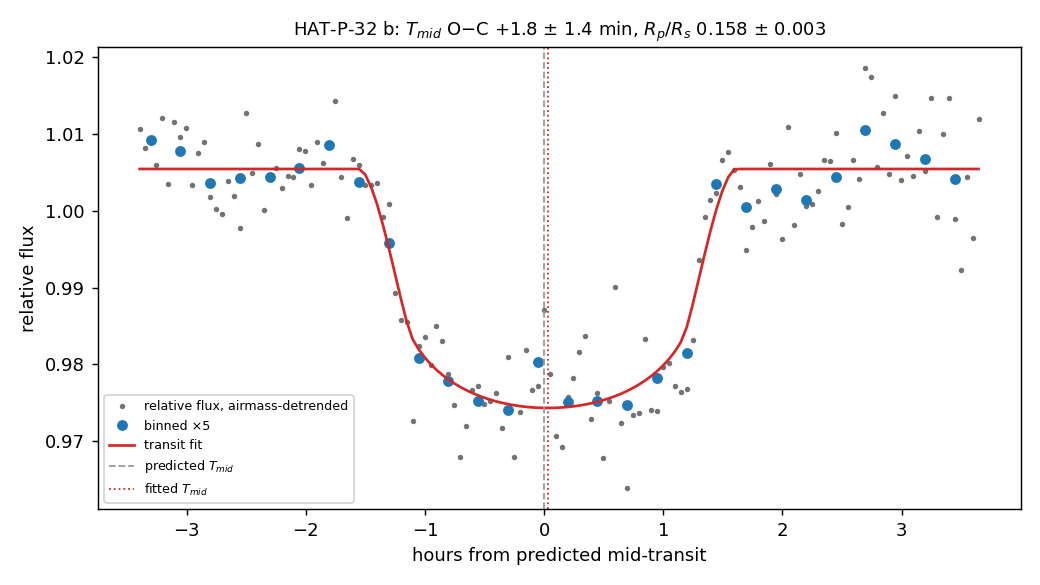
\includegraphics[width=0.8\textwidth]{figs/hatp32.png}
\caption{HAT-P-32\,b relative light curve (grey points) with the fitted
transit model (red), from the reduction with a photometric aperture radius
of $1.4\times$FWHM (\SI{3.5}{px}). The x-axis is hours from the
mid-transit time predicted by the published ephemeris (grey dashed line);
the red dotted line is the fitted $T_\mathrm{mid}$, \SI{1.75}{min} after
that prediction and \SI{1.9}{min} before EXOTIC's result for this night.
The fitted $R_p/R_s$ is 0.158 (Table~\ref{tab:hatp32}).}
\label{fig:hatp32}
\end{figure}

\subsection{WASP-36\,b}

55 frames of \SI{60}{s}. Plate solving and frame alignment worked, but the
target ($G=12.6$) is limited by sky noise: the best scatter is 2.3\% per
point, with a photometric aperture radius of $1.0\times$FWHM (\SI{2.3}{px}).
Scatter fell steadily with smaller apertures, as expected for a faint star
dominated by sky noise (6.2\% at the default $1.9\times$FWHM). The transit
is ${\sim}1.8\%$ deep. The fit (Figure~\ref{fig:wasp36}) gives
$T_\mathrm{mid}$ $+15.4\pm\SI{6.3}{min}$ from the ephemeris prediction and
$R_p/R_s=0.152\pm0.022$ (literature 0.134). Treat this as provisional. A
66-minute gap leaves only 3 frames before ingress, so the out-of-transit
level is set almost entirely after egress, and a timing offset of
$2.4\sigma$ may well be systematic. With the default $1.9\times$FWHM
aperture the fit gives $-30\pm\SI{27}{min}$ and $0.17\pm0.07$.

\begin{figure}[ht]
\centering
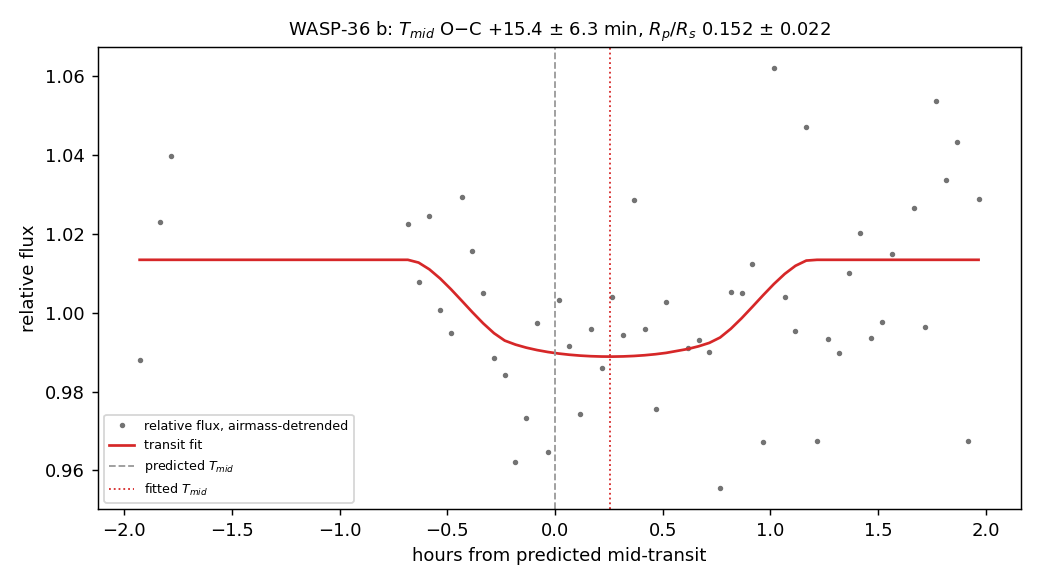
\includegraphics[width=0.8\textwidth]{figs/wasp36.png}
\caption{WASP-36\,b relative light curve (grey points) with the fitted
transit model (red), from the reduction with a photometric aperture radius
of $1.0\times$FWHM (\SI{2.3}{px}). The dashed grey
line is the predicted mid-transit time and the dotted red line the fitted
one. Only three points precede the transit.}
\label{fig:wasp36}
\end{figure}

\subsection{POTS-1\,b, WFI}\label{sec:pots1}

\begin{itemize}
  \item \textbf{Calibration:} gain and read noise were measured for each
        detector from bias and flat pairs, because the headers record gain
        for only two detectors and read noise for none. Gain came out at
        1.94--\SI{2.28}{e^-/ADU} and read noise at 5.6--\SI{6.2}{e^-},
        consistent with WFI's documented values.
  \item \textbf{Astrometry:} all 8 detectors plate-solved, with 36--163
        Gaia stars each and residuals of 0.06--\SI{0.11}{arcsec}. POTS-1 is
        on chip 3.
\end{itemize}

\paragraph{First extraction (failed).}
801 stars down to $G=18.5$ were photometered across all 310 frames, with
a photometric aperture radius of $1.9\times$FWHM (\SI{10.1}{px}). The
result is shown for information in Figure~\ref{fig:pots1first}. The
target's relative light curve scatters by 27\% from point to point. That's
far above the ${\sim}1\%$ photon noise expected for a $G=17.2$ star in a
\SI{26}{s} exposure on a \SI{2.2}{m} telescope, and it swamps the
${\sim}2.5\%$ transit. Every star on the chip is affected: scatter is
1.8\% at $G=12$, 4.4\% at $G=15$ and over 20\% at $G\geq17$, against
predicted uncertainties of 0.06--0.9\%. Star tracking was fine: the target
stays within \SI{0.4}{px} of the comparison stars.

There were two causes:
\begin{itemize}
  \item \textbf{Sky background (EXOTIC).} \texttt{skybg\_phot} takes the
        sky level as the statistical \emph{mode} of the pixel values in a
        box around each star. The box includes the star itself, not just
        the annulus. On raw integer frames (MicroObservatory) the mode
        works, which is why HAT-P-32 validates. On bias- and
        flat-corrected frames, which are floating point, almost every
        value is unique, so the ``mode'' is an arbitrary pixel. For the
        target it jumped between 28 and 62\,ADU from frame to frame, against
        a true sky of ${\sim}50$\,ADU. Over the 320-pixel aperture that is
        a 20--30\% flux error. Workaround: round calibrated frames to
        whole ADU before extraction. That adds 0.3\,ADU of rounding noise
        against 7\,ADU of sky noise.
  \item \textbf{Fixed orbit (ours).} The NASA Exoplanet Archive has no
        tabulated $a/R_s$ for POTS-1\,b, and the code defaulted it to
        zero, so the transit model was degenerate (hence the infinite
        uncertainty in Figure~\ref{fig:pots1first}). It is now derived from
        the semi-major axis and the stellar radius.
\end{itemize}

\begin{figure}[ht]
\centering
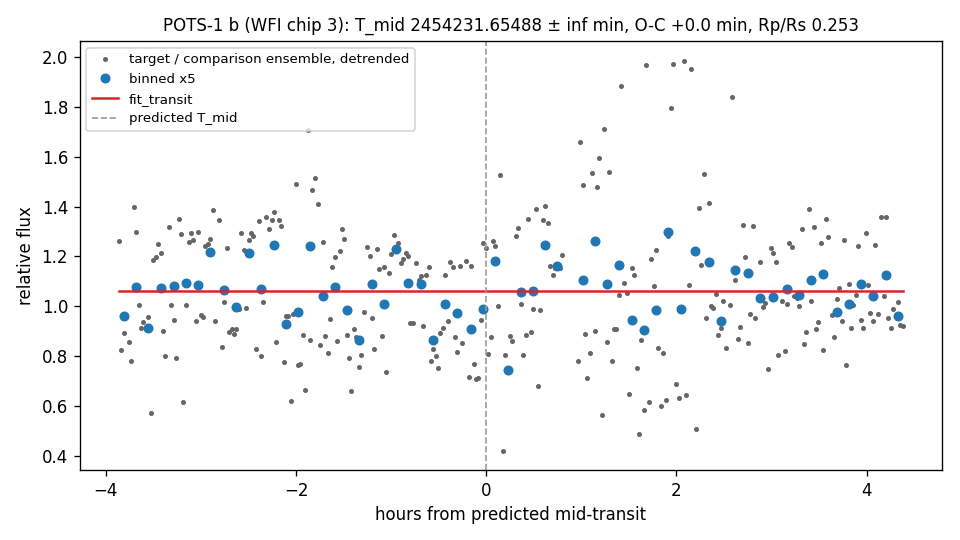
\includegraphics[width=0.8\textwidth]{figs/pots1_first_run.png}
\caption{First, failed extraction of POTS-1\,b (WFI chip 3), shown for
information. Grey points are the target's relative flux per frame, blue
points are 5-frame bins, and the red line is the failed fit. The 27\%
point-to-point scatter comes from the unstable sky-background estimate on
calibrated (floating-point) frames. The fit is meaningless because $a/R_s$
was zero. Both problems are fixed in the re-run.}
\label{fig:pots1first}
\end{figure}

\paragraph{Corrected extraction.}
Re-run with both fixes at two photometric aperture radii. Each run takes
${\sim}\SI{30}{min}$ on 12 cores. Ephemeris and catalogue values are from
the NASA Exoplanet Archive. Note that these WFI data are the survey in
which POTS-1\,b was discovered, so this tests whether we recover a known
result, not an independent detection.

\begin{table}[ht]
\centering
\caption{POTS-1\,b transit fits from WFI chip 3 (310 frames, 801 stars
photometered) for two photometric aperture radii. \emph{$T_\mathrm{mid}$
offset} is relative to the ephemeris prediction (uncertainty
\SI{0.6}{min}). \emph{Fitted $R_p/R_s$} is the planet-to-star radius ratio;
the catalogue value is 0.164. \emph{Scatter} is the rms of the fit
residuals. \emph{Clipped} is the number of frames
dropped as $>4\sigma$ outliers.}
\label{tab:pots1}
\begin{tabular}{cccccc}
\toprule
\multicolumn{2}{c}{Photometric aperture radius} & Scatter & $T_\mathrm{mid}$ offset & Fitted $R_p/R_s$ & Clipped \\
($\times$FWHM) & (px) & & (min) & (planet / star) & \\
\midrule
1.2 & 6.4 & 2.3\% & $+4.7\pm4.0$ & $0.166\pm0.010$ & 2 \\
1.9 & 10.1 & 4.1\% & $+5.8\pm7.6$ & $0.159\pm0.018$ & 3 \\
\bottomrule
\end{tabular}
\end{table}

Both reductions recover the transit at the predicted time (within
$1.2\sigma$) and with the catalogue depth (Table~\ref{tab:pots1},
Figure~\ref{fig:pots1}). The smaller aperture halves the scatter, as for
the faint MicroObservatory target. Frames between about +1 and +3\,h after
mid-transit are noisier than the rest; the cause (transparency, or a
neighbouring star) hasn't been checked yet.

\begin{figure}[ht]
\centering
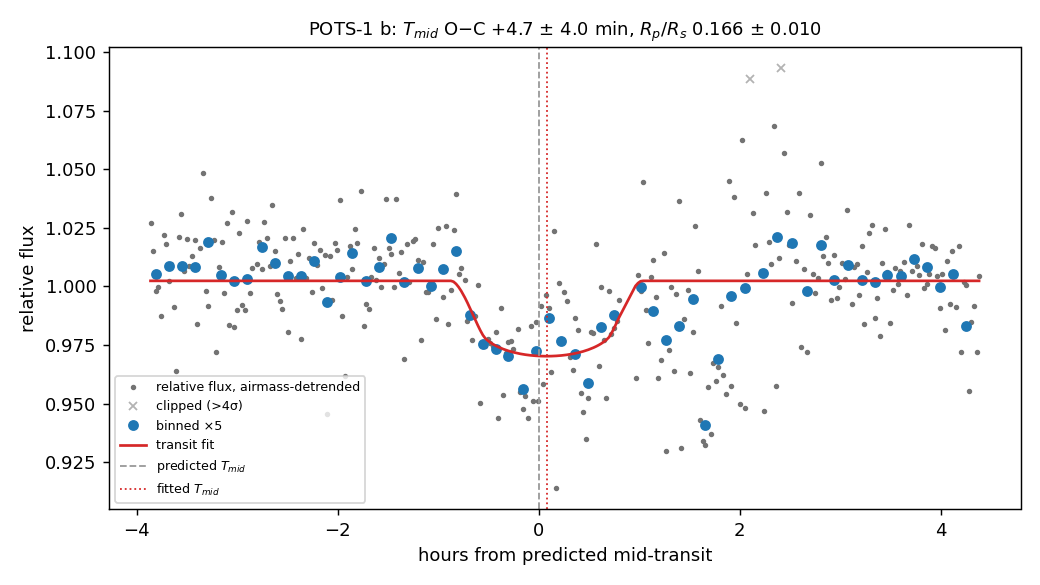
\includegraphics[width=0.85\textwidth]{figs/pots1.png}
\caption{POTS-1\,b relative light curve from WFI chip 3 with a photometric
aperture radius of $1.2\times$FWHM (\SI{6.4}{px}). Grey points are single
\SI{26}{s} frames, blue points 5-frame bins, crosses frames clipped as
$>4\sigma$ outliers. The red line is the transit fit. The grey dashed and
red dotted lines mark the predicted and fitted mid-transit times.}
\label{fig:pots1}
\end{figure}

\section{Issues and next steps}\label{sec:issues}

\begin{itemize}
  \item \textbf{Speed:} centroid fitting in \texttt{extract\_frame} takes
        ${\sim}\SI{70}{ms}$ per star per frame, which dominates run time
        (about \SI{55}{s} per WFI frame for 800 stars). Running in parallel
        works around it for now. This is a useful benchmark for the GPU
        work in EXOTIC.
  \item \textbf{EXOTIC sky background:} \texttt{skybg\_phot}'s modal
        estimate fails on calibrated, floating-point frames (Section~\ref{sec:pots1}).
        We work around it by rounding, but the proper fix belongs in
        EXOTIC: estimate the sky from the annulus pixels only, with a
        sigma-clipped median, so it works whatever the data type. EXOTIC's
        own pipeline is affected whenever it applies darks or flats.
  \item \textbf{EXOTIC quick fit at absolute BJD:} \texttt{quick\_fit.fit\_transit}
        passes BJD ($\sim2.45\times10^6$) straight to \texttt{curve\_fit},
        whose finite-difference step scales with the parameter value. The
        step on $T_\mathrm{mid}$ is then about \SI{50}{min}, wider than the
        ingress. On the noisy POTS-1 data the fit stalled at its starting
        values. On HAT-P-32 and WASP-36 it converged only partly and
        overstated its uncertainties. Earlier numbers in this report have
        been refitted. Fix used here: fit times relative to the start of
        the night, from a grid-search start. It would be simple to do the
        same inside \texttt{fit\_transit}.
  \item \textbf{Photometric aperture size:} the default FWHM-scaled aperture is too large
        for faint, sky-limited stars. It should be tuned per star, or chosen
        by sweeping, for bycatch at scale.
  \item \textbf{Limb darkening:} fixed approximate coefficients bias the
        fitted $R_p/R_s$. Timing is unaffected.
  \item \textbf{Next:} check the noisy interval in the POTS-1 light curve;
        run the remaining MicroObservatory targets; look for variability among the field stars in the JSON
        results; then scale the search to OmegaCAM and the other WFI
        sequences.
\end{itemize}

\end{document}
